% Section 1: Setting up the environment
\newpage
\section{Setting up the environment}
Typical programming in Python heavily relies on external packages, which can have different versions and dependencies. To avoid conflicts between different projects, it is recommended to use a virtual environment for each project. We will be using such a virtual environment in this course to ensure a consistent development environment for everyone. Virtual environments are the recommended way to manage dependencies in Python projects.

To manage these virtual environments we will be using the open-source tool \verb|uv|, available from \url{https://github.com/astral-sh/uv}. If you have any version of Python already installed, you can install uv by simply running
\begin{lstlisting}
pip install uv
\end{lstlisting}
If you don't have Python installed, you can download it from \url{https://www.python.org/downloads/} and then use the above command or use the stand-alone installers on \url{https://github.com/astral-sh/uv}.

To test the installation, run in your command line
\begin{lstlisting}
uv --version
\end{lstlisting}
and something similar to \verb|uv 0.5.30| should appear.

Now we will create a project called \verb|NOFY080_2025| that will hold all the files related to this course, run
\begin{lstlisting}
uv init NOFY080_2025
\end{lstlisting}
which will create a new directory with the same name, with a simple "Hello World" Python file, some additional files that \verb|uv| uses to track dependencies of your project, and set up a git repository in it (you don't have to use git in this course, but those interested can learn some basics in Appendix~\ref{sec:git}).

Now change into the project directory
\begin{lstlisting}
cd NOFY080_2025
\end{lstlisting}
and add packages that we will need throughout this course
\begin{lstlisting}
uv add numpy scipy matplotlib
\end{lstlisting}
which will create the virtual environment and install the specified packages (a directory \verb|.venv| should appear in the project directory).

If you wanted to create a virtual environment without installing any packages, you could use the command
\begin{lstlisting}
uv venv <name of the virtual environment>
\end{lstlisting}

To activate the virtual environment, run the following command on Linux or Mac OS
\begin{lstlisting}
source .venv/bin/activate
\end{lstlisting}
and on Windows
\begin{lstlisting}
.venv\Scripts\activate
\end{lstlisting}

Now, when you run \verb|python|, the virtual environment version will be run, rather than your system version. To deactivate the virtual environment, simply run \verb|deactivate|.

\subsection{Running Python code}
Python is an interpreted language that does not need to be compiled before it is run. We save Python code in text files with the \verb|.py| file extension or in so-called Jupyter notebooks (file extension \verb|.ipynb|).

To test our installation, create a new Python file (a text file with the suffix \verb|.py|) \verb|test.py| in our project directory with the following content
\begin{lstlisting}
import matplotlib.pyplot as plt

plt.plot([1, 2, 3], [4, 5, 6], '-o')
plt.show()
\end{lstlisting}
To run it, you can either manually activate the virtual environment and run it using
\verb|python test.py| or use \verb|uv run test.py|. A simple graph should appear. In the rest of these lecture notes, whenever we invoke \verb|python| command from the command line, we mean the one in the virtual environment.

To run Python code directly without saving it to a file, open a suitable terminal and type in \verb|python| and a prompt like
\begin{lstlisting}
    >>>
\end{lstlisting}
will appear. This is the Read-Evaluate-Print-Loop (REPL); any code entered will be run and the result printed on the screen. To exit, enter \verb|quit()|. To execute a file \verb|myfile.py|, first navigate to its directory and then run it simply with \verb|python myfile.py| (note that if you have your virtual environment activated, the actual Python script does not have to be located in your project directory).

\begin{exercise}
    Create a text file \verb|hello.py| which contains a single line
    \begin{lstlisting}
        print("Hello world!")
    \end{lstlisting}
    and then run this file.
\end{exercise}

Sometimes we do not want the Python interpreter to quit immediately after finishing running our program (e.g., we want to inspect variables created during the program run); this can be done using \verb|python -i file.py|, where \verb|-i| stands for \emph{interactive}. Alternatively, a more user-friendly (color-coded syntax, auto-completion, etc.) version of the interactive Python REPL can be invoked using \verb|ipython| (or \verb|ipython3|, depending on your installation), which can also be used to interactively run files using \verb|ipython3 -i myfile.py|.

\subsection{A quick note on text editors}
Any text editor can be used to write Python code, including the default Windows Notepad. However, it is beneficial to your mental health to use at least something with syntax highlighting, such as Notepad++, or a more feature-rich editor such as VS Code or Spyder where you can run your file without switching to a terminal. In this course, I recommend using VS Code with the Python extension installed, because it makes working with virtual environments easier. Opening a directory in VS Code will automatically detect the virtual environment and use it when the file is run. The name of the virtual environment currently used is indicated in the bottom right corner (highlighted in red):
\begin{center}
    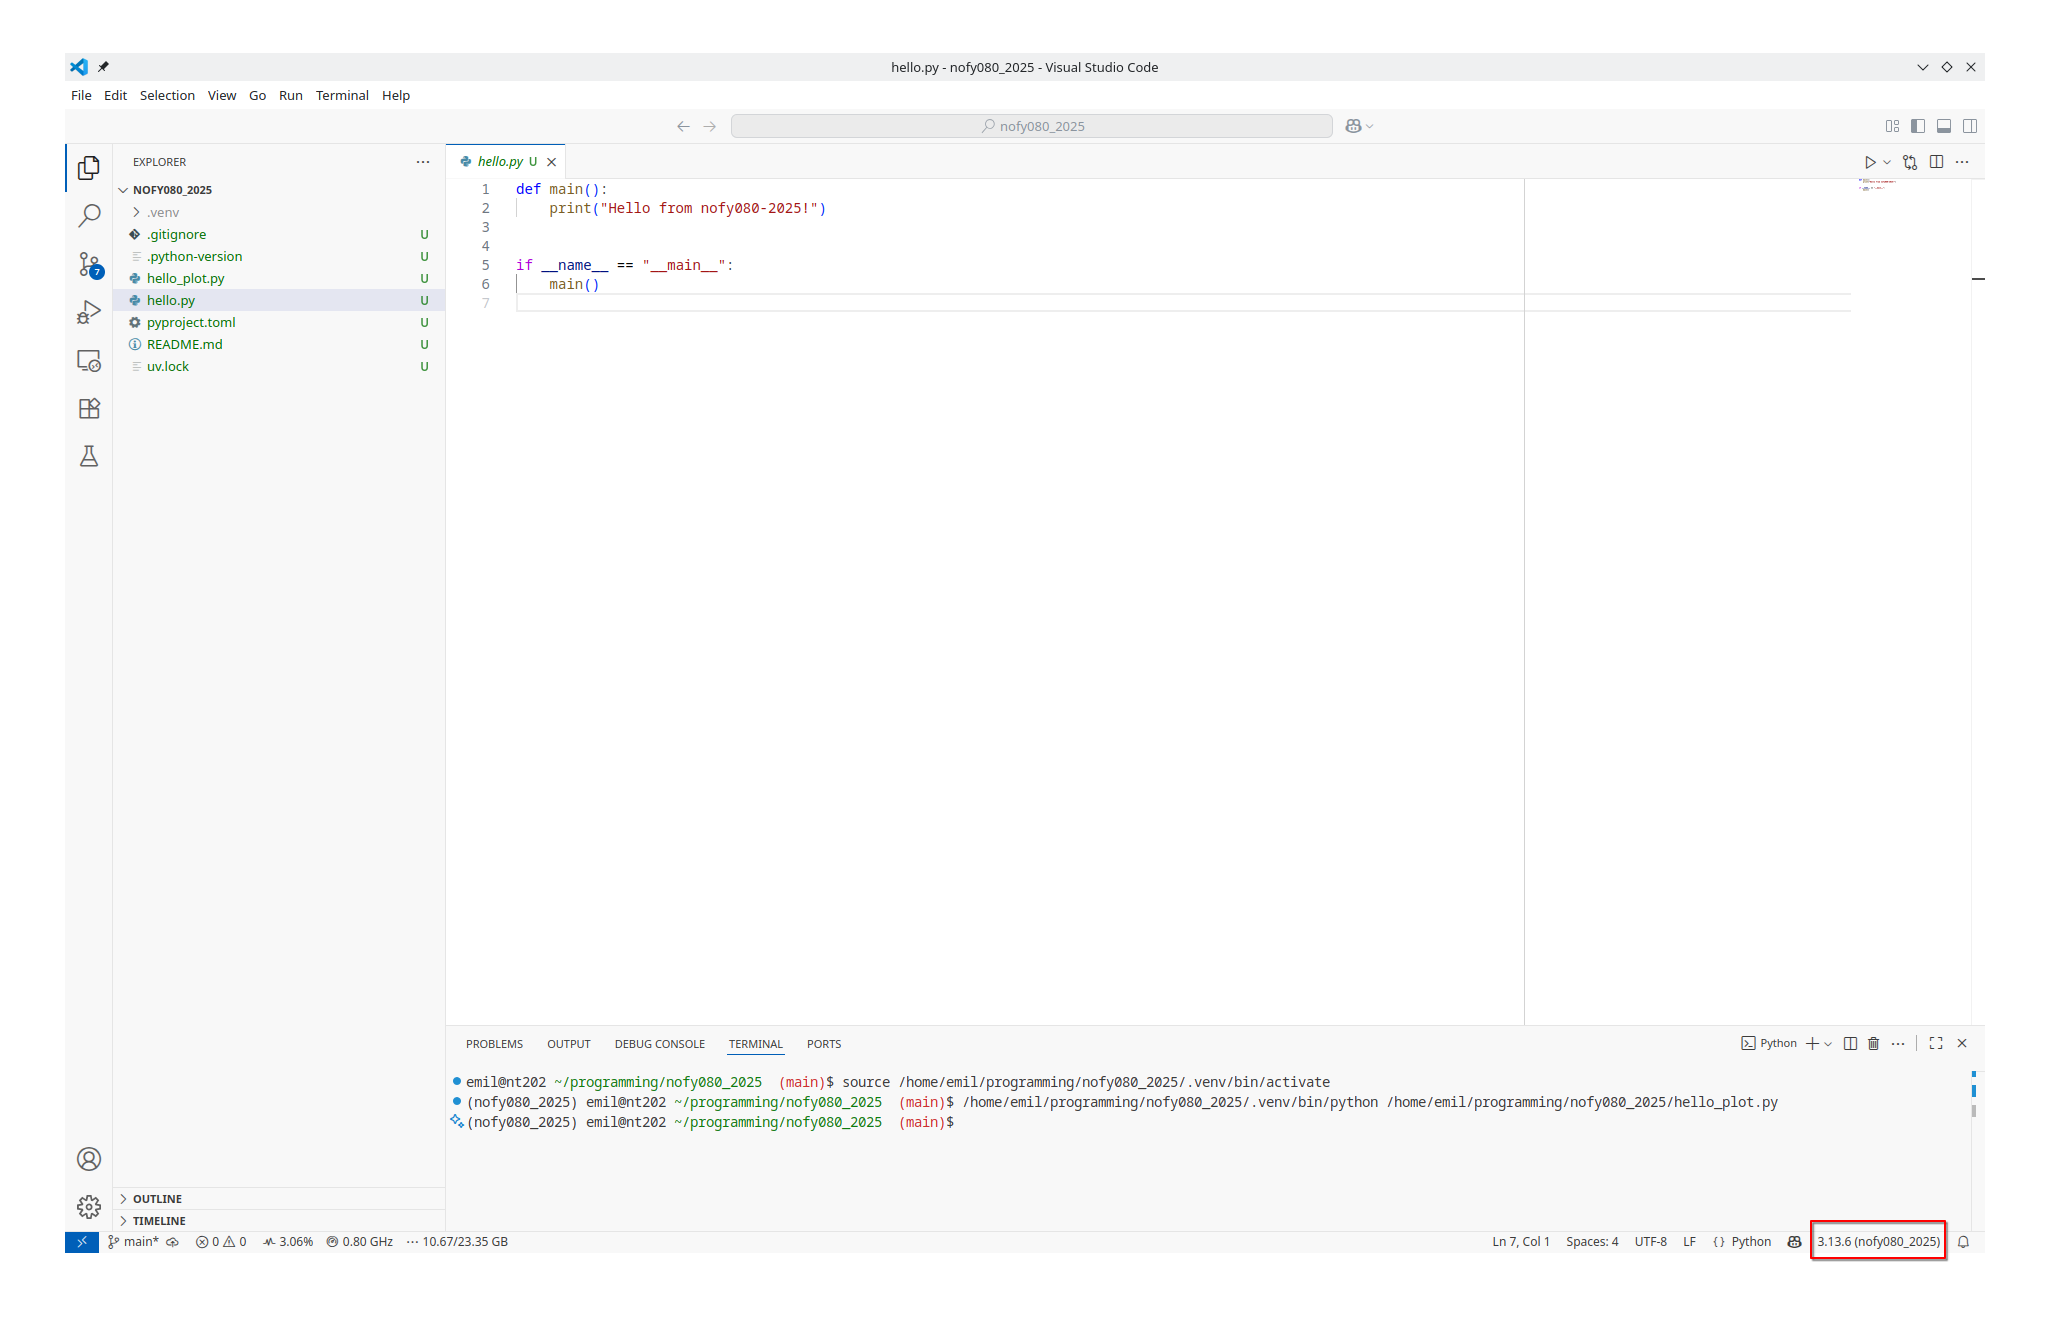
\includegraphics[width=0.9\linewidth]{vscode.png}
\end{center}

Working with environments in Spyder is somewhat more involved; see the guide \href{https://github.com/spyder-ide/spyder/wiki/Working-with-packages-and-environments-in-Spyder#working-with-other-environments-and-python-installations}{here}.

\subsubsection{Jupyter Notebooks}
Jupyter notebooks (run using \verb|jupyter-notebook| in the command line) provide an easy-to-use interactive environment with an interface running in a web browser. They are good for trying things out\footnote{In this course we will be (mostly) using scripts due to easier splitting into modules and fewer issues with parallel programming, which we will encounter later on.}. Jupyter notebooks also work well with virtual environments and VS Code. Navigate to your project directory and run
\begin{lstlisting}
uv pip install jupyter ipympl
\end{lstlisting}
The \verb|ipympl| package enables the use of interactive Matplotlib plots in Jupyter notebooks. Next, also install the \verb|jupyter| extension in VS Code. Now simply create a file with the extension \verb|.ipynb| and you can use it within VS Code as you would in the browser. On the first run, you will be asked to pick the virtual environment in which the notebook should run; the one we created should be one of the options if the notebook is saved in the project directory (same directory as the \verb|.venv| directory).

\begin{center}
    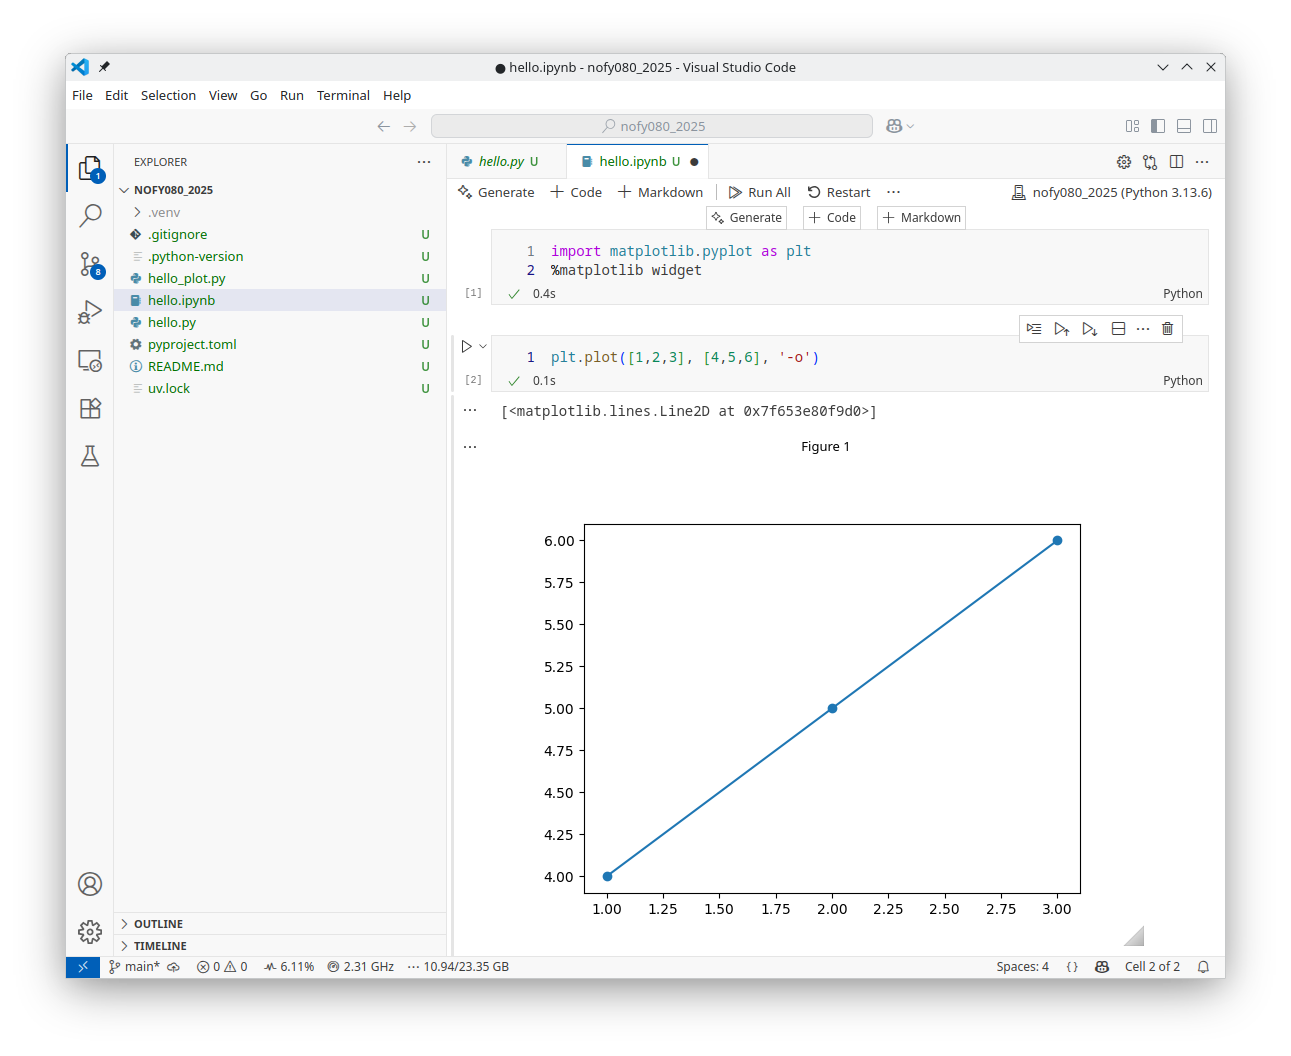
\includegraphics[width=0.9\linewidth]{vscode_jupyter.png}
\end{center}